\documentclass[conference]{IEEEtran}
\IEEEoverridecommandlockouts
% The preceding line is only needed to identify funding in the first footnote. If that is unneeded, please comment it out.
\usepackage{cite}
\usepackage{amsmath,amssymb,amsfonts}
\usepackage{algorithmic}
\usepackage{graphicx}
\usepackage{textcomp}
\usepackage{xcolor}
\usepackage[binary-units=true]{siunitx}
\usepackage{subcaption}
\def\BibTeX{{\rm B\kern-.05em{\sc i\kern-.025em b}\kern-.08em
    T\kern-.1667em\lower.7ex\hbox{E}\kern-.125emX}}
\begin{document}

\title{Learning to detect robots from artificial images\\
%{\footnotesize \textsuperscript{*}Note: Sub-titles are not captured in Xplore and
%should not be used}
\thanks{Identify applicable funding agency here. If none, delete this.}
}

\author{\IEEEauthorblockN{1\textsuperscript{st} Christoph Heindl}
\IEEEauthorblockA{\textit{Visual Computing} \\
\textit{PROFACTOR GmbH}\\
4407 Steyr, Austria \\
christoph.heindl@profactor.at}
\and
\IEEEauthorblockN{2\textsuperscript{nd} Sebastian Zambal}
\IEEEauthorblockA{\textit{Machine Vision} \\
\textit{PROFACTOR GmbH}\\
4407 Steyr, Austria \\
sebastian.zambal@profactor.at}
%%%\and
%%%\IEEEauthorblockN{3\textsuperscript{rd} Markus Ikeda}
%%%\IEEEauthorblockA{\textit{Robotics} \\
%%%\textit{PROFACTOR GmbH}\\
%%%4407 Stey, Austria \\
%%%markus.ikeda@profactor.at}
%%%\and
%%%\IEEEauthorblockN{~~~~~~~~~4\textsuperscript{th} Christian Eitzinger~~~~~~~~~}
%%%\IEEEauthorblockA{\textit{Machine Vision} \\
%%%\textit{PROFACTOR GmbH}\\
%%%4407 Stey, Austria \\
%%%christian.eitzinger@profactor.at}
%%%\and
%%%\IEEEauthorblockN{5\textsuperscript{th} Andreas Pichler}
%%%\IEEEauthorblockA{\textit{Robotics} \\
%%%\textit{PROFACTOR GmbH}\\
%%%4407 Stey, Austria \\
%%%anreas.pichler@profactor.at}
\and
\IEEEauthorblockN{6\textsuperscript{th} Josef Scharinger}
\IEEEauthorblockA{\textit{Institute of Computational Perception} \\
\textit{Johannes Kepler University}\\
4040 Linz \\
josef.scharinger@jku.at}
}

\maketitle

\begin{abstract}
Impressive results have been achieved in computer vision via machine learning methods over the last years. However, for many highly specialized industrial applications these methods cannot directly be applied due to the lack of large amounts of training data. In this paper we propose a software framework that provides artificial data. Such artificial data opens the door for machine learning even when it is hard or impossible to acquire real data. The presented system is flexible in the sense that it supports image data generation in a flexible way. We show how artificial images can directly be used in pytorch to perform deep neural network training. 
\end{abstract}

\begin{IEEEkeywords}
machine learning, artificial data, data augmentation
\end{IEEEkeywords}

\section{Introduction and Related Work}
The impressive results of supervised deep learning in the field of robotics and computer vision are to large extent due to the availability of annotated data sets. Up until recently most of the annotation was carried out by domain experts. This time consuming process significantly slows down the progress of deep learning efforts. In many tasks it is difficult, in most niche areas impossible, to obtain strong supervision because of the high costs.

Exposed to this bottleneck, new fields of research have opened up. Active learning \cite{druck2009active, settles2012active, cakmak2012designing} attempts to use human experts in a more targeted way by focusing on samples that seem to of highest value for learning task. Semi-supervised learning \cite{chapelle2009semi, salimans2016improved, zhu2006semi} combines large unlabeled data sets with smaller labeled data sets through structural assumptions, such as smoothness or low-dimensionality constraints. Transfer learning \cite{pratt1993discriminability, ventura2007theoretical, pan2010survey} exploits the fact that models trained on specific tasks can be adapted to related problems using fewer training samples. Weak supervision \cite{ratner2016data, zhou2017brief} is motivated by leveraging less precise, higher level supervision that is often easier to obtain. This includes heuristics, weak or biased classifiers, unreliable non-experts. 

% https://hazyresearch.github.io/snorkel/blog/ws_blog_post.html

In contrast to the methods mentioned above, synthetic data generation drops the necessity for real world annotated data in favor of artificial data sources. Synthesized data is available in virtually infinite variety and is de-facto auto-labelled. This has led to variety of successful applications in different domains: Jaderberg et al. \cite{jaderberg2014synthetic} have demonstrated natural scene text recognition from synthetic data, Peng et al. \cite{peng2015learning} trained object detectors from 3D models and Johnson et al. \cite{2017_Johnson_DrivingInTheMatrix} used photo-realistic computer rendering captured from a game engine to train car detectors. 

A common theme to all of these synthetic approaches is the following: (a) a simulator engine generators artificial training data, (b) the generated data is stored to disk and (c) the offline data stack is used for training. The shortcomings to this procedure are early training data commitment and the lack of adaptability of data generation to training demands.

In this paper we propose method of generating artificial training data from a simulator engine that is directly looped into the training procedure, thereby avoiding early data commitment. A bi-directional communication channel enables adaptive random data generation. We demonstrate the usefulness of our approach to the detection of robot poses in color images trained from non-realistic computer generated images.


%\begin{figure}[htbp]
%\centerline{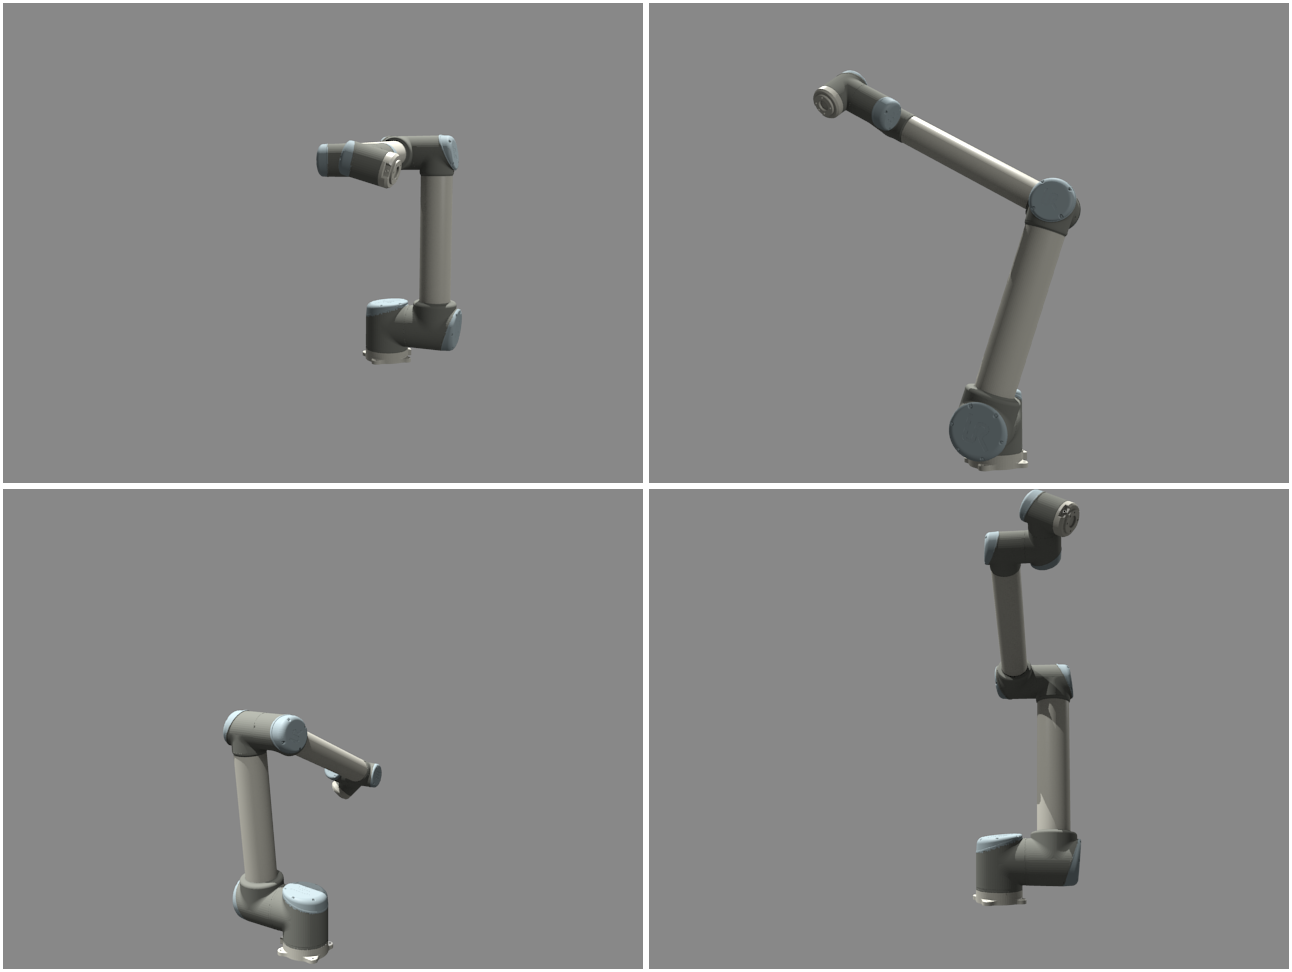
\includegraphics[width=\columnwidth]{figures/examplesUR10/renderedImages.png}}
%\caption{\label{fig:architecture} Architecture of our system: Individual instances generate artificially %rendered images (left). These are consumed in a pytorch environment for training of deep neural networks %(right).}
%\label{fig}
%\end{figure}


\section{Method}

    Our approach is outlined in Figure \ref{fig:architecture}. Without loss of generality we consider a supervised regression task. One or more simulator engines generate training tuples $\{(\textbf{x},y,\textbf{h})\} \sim P(\textbf{X},Y,\textbf{H};\theta)$ by sampling from a probabilistic graphical model parametrized by $\theta$. The training samples $\{(\textbf{x},y)\}$ are used for mini-batch updating the parameters $\phi$ of a neural network $P(Y \lvert \textbf{X};\phi)$. Finally, the simulation parameters $\theta$ are adapted via a feedback signal emitted from control unit.

    \begin{figure}[htbp]
        \centerline{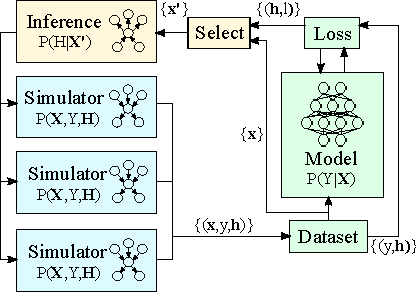
\includegraphics[width=0.9\columnwidth]{figures/architecture/overview.pdf}}
        \caption{\label{fig:architecture} Architecture of our system.}
    \end{figure}


\subsection{Artificial data and data loaders}

TODO: Outline Python-support of Blender, Explain scripting in Blender, creation of meta-data (joint locations, etc.)...
TODO: Explain basic concepts of PyTorch and DataLoaders, etc.
TODO: Explain ZMQ pipeline, publish/subscribe

\subsection{Localization Model and Training}

    Joint localization deals with the task of estimating positions of articulated body parts that constitute kinematic chains. In this work, we define joint localization to be the process of predicting 2D pixel coordinates of robotic revolute joints from color image input. 
    
    Our model, outlined in Figure \ref{fig:jointmodel}, is based on the architecture proposed by Heindl et al. \cite{cheind2019disp}, which in turn is an extension to methods developed for human pose estimation \cite{cao2017realtime, newell2016stacked}.  . Instead of predicting sparse joint pixel coordinates, we train the network to predict dense belief maps per joint $\hat{\mathbf{B}} \in \mathbb{R}^{J \times H' \times W'}$ in the following way. Color images $\mathbf{I} \in \mathbb{R}^{3 \times H\times W}$ are input to a pre-trained VGG network \cite{simonyan2014very} to extract base features $\mathbf{F} \in \mathbb{R}^{C \times H' \times W'}$. A series of convolutional image-to-image networks refines belief predictions by allowing each network to work on the basis of outputs from the previous network and VGG base features.

    \begin{figure} [!h]
        \centering
        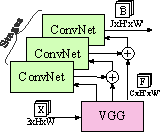
\includegraphics[width=0.7\columnwidth]{figures/joint_model/joint_model.pdf}
        \caption {
            \label{fig:jointmodel} 
            Architecture of the localization module. Each stage predicts joint belief maps. Successive stages are fed a channel concatenated stack of VGG features and the current estimate.
        }
    \end{figure}

    We generate target belief maps $\mathbf{B}$ by pixel-wise maximization over the contributions from $J$ squared exponential kernels
    \begin{equation}
        k_{\textrm{SE}}(\mathbf{x};\mathbf{z}) = \sigma^2e^{-\frac{\lVert \mathbf{x} - \mathbf{z} \rVert^2_2}{l^2}}
    \end{equation}
    centered at sparse image joint locations $\{\mathbf{z}_0,\ldots,\mathbf{z}_J\}$. The output variance $\sigma^2$ determines the average distance away from its mean, the length-scale $l$ determines the width of the kernel. During training, a objective functions after each stage penalizes pixel-wise differences between belief predictions $\hat{\mathbf{B}}$ and targets $\mathbf{B}$. Usually, $L_2$ or smooth $L_1$ loss functions are used. These intermediate losses help the network to train more effectively, as the effect of vanishing gradients in deep architectures is minimized \cite{newell2016stacked, wei2016convolutional}. 
    
    When predicting from the network only the output of the last stage is used. For partial scale invariance of image features, we additionally average the belief predictions of input images scaled to different resolutions.

\subsection{Feedback Mechanism}
    \label{sec:feedback}
    A key idea to our work is a feedback mechanism that enables adaptive sampling from simulator engines. As outlined in Figure \ref{fig:architecture}, a controller updates the simulation based on information of the current training mini-batch. The update can be in principle of any kind, however, in this work we focus on modifying probability distributions of the graphical model controlling the simulation process. In particular we modify distributions of hidden variables in such a way that more examples $\{(\textbf{x},y,\textbf{h})\}$ of high value to the training are produced. Once a subset of important examples $\mathcal{S} = \{(\textbf{x},y,\textbf{h})\}$ from the training batch has been selected, we infer $P(\textbf{H},Y \lvert \textbf{X};\mathcal{S})$ (approximately, analytically or in a heuristic fashion) and continue sampling from the updated distribution.

    We propose two ways to measure the value of specific samples for training. The first utilizes the loss function to assign more importance to examples of high error. This trivially leads to updated sampling strategies putting more weight into regions of high training error. The second method uses prediction uncertainty to select sample candidates. In contrast to Bayesian learning for neural networks \cite{neal2012bayesian}, deterministic regression networks do not have any meaningful measure of uncertainty build in or are not well calibrated for uncertainty estimation (in the classification case) \cite{guo2017calibration}. One way to overcome this limitation is perform approximate Bayesian uncertainty estimation as proposed in Gal et al. \cite{gal2015dropout}. Samples selected by uncertainty are intrinsically determined by the model without consulting a loss function.
    
    %http://stillbreeze.github.io/Uncertainty-Estimation-in-Deep-Learning/

\subsection{Implementation Notes}
    We use Blender \cite{blender} as a simulator engine for robotic scenes. Blender offers great scripting support, that allows us to hook into the rendering process. Our localization model is defined and trained using PyTorch \cite{paszke2017automatic}. As communication layer we use the distributed messaging library ZeroMQ \cite{zeromq_guide}. In particular, publisher/subscriber patterns are used for broadcasting simulation results to the training loop. We limit the number of outstanding messages at the subscriber to prevent the training loop from running out of memory. The control signal is based a simple request/reply pattern. As outlined in figure \ref{fig:architecture}, TCP/IP is used as transport layer. 

\section{Results}

    In the following we describe the training procedure, evaluation of our method on synthetic and real world data, and provide runtime metrics.

    \subsection{Training}
    For training the localization model we sampled a set of 10.000 samples per epoch from two simulator engines. The first simulator generated uniform random poses, while the second simulator produced importance samples as described in Section \ref{sec:feedback} according to a loss metric. Two distinct collections of random background images (city and industrial theme) were used as synthetic training- and test-set backgrounds. We trained the joint localization model using six stages with input images of size $320 \times 240$. A VGG network, pre-trained on detection, was used to generate base features. We used Adam \cite{kingma2014adam}, $\eta=\num{1e-3}$, optimization with mini-batch learning for a total of 30 epochs.

    \subsection{Evaluation}
    We challenge joint localization model trained on artificial images on synthetic and real world image. For comparison we extract joint locations from prediction belief maps $\hat{\mathbf{B}}$ by performing smoothed non-maximum suppression, followed by extracting the maximum peak per joint channel. For real-world images we asked a human export to annotate the joint locations. Synthetic images are auto-labelled by our simulation engine. We define the localization error to be the Euclidean distance between predicted and target pixel locations and report it in percent of image diagonal. 
    
    Figure \ref{fig:pixelerror} shows the localization error on two distinct test sets: synthetic with random backgrounds (Figure \ref{fig:locationerror_synth}) and real-world images (Figure \ref{fig:locationerror_real}). As expected our system performs better on synthetic data than real data. 

    \begin{figure}[!h]
        \centering
        \begin{subfigure}[t]{0.49\columnwidth}
            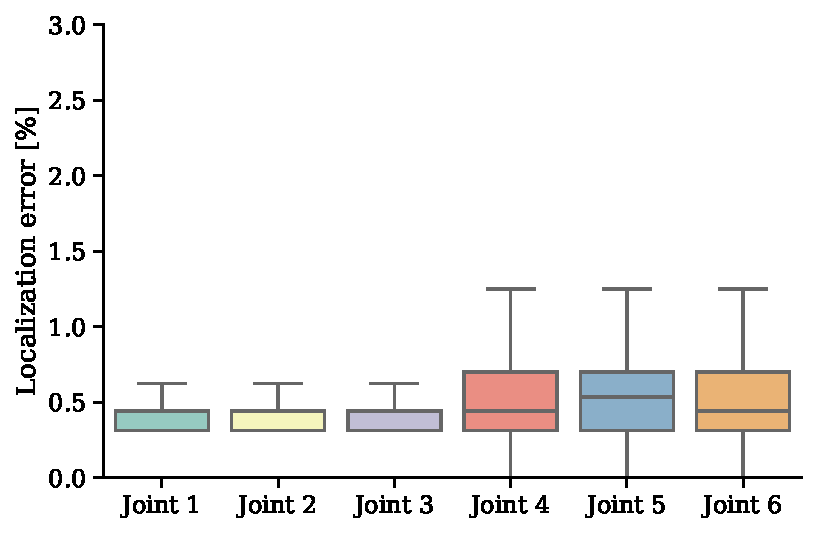
\includegraphics[width=\columnwidth]{figures/results/pixel_errors/pixel_error_synth.pdf}
            \caption {
                \label{fig:locationerror_synth} 
                Localization errors of joint prediction on a synthetic test data set with auto-labelled ground truth.
            }
        \end{subfigure}
        \begin{subfigure}[t]{0.49\columnwidth}
            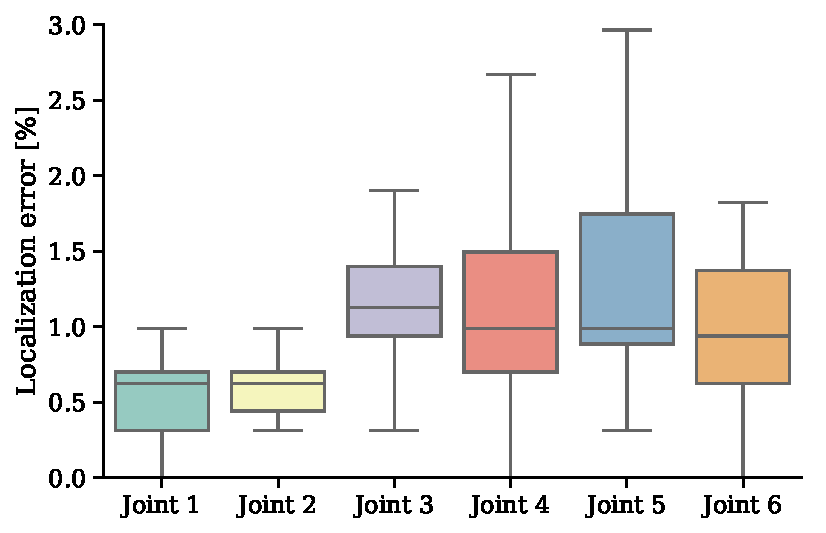
\includegraphics[width=\columnwidth]{figures/results/pixel_errors/pixel_error_real.pdf}
            \caption {
                \label{fig:locationerror_real} 
                Localization errors of joint prediction for a real world test set. Target locations annotated by a human domain expert. 
            }
        \end{subfigure}
        \caption {
            \label{fig:pixelerror} 
            Localization errors of robot joint prediction. Results are in percent of image diagonal.
        }
    \end{figure}

    We attribute two effects for this outcome: (a) our simulation is non-realistic and (b) human annotation is error-prone. To underpin the latter issue, we have conducted a pilot study in which 10 people (all with reference to robotics) annotated 12 real world images of an UR-10 robot in different poses and from different viewpoints. We than computed the inter-rater spread as measure of confidence for human annotations in our domain. Figure \ref{fig:humanuncertainty} shows the average uncertainty per joint over all images. We find that the middle joints, often blocked by view and robot pose, are the most difficult to annotate precisely. The results indicate that our method performs better than indicated by figure \ref{fig:locationerror_real}, because this figure does not take into account human annotation errors.

    \begin{figure}[!h]
        \centering
        \begin{subfigure}[t]{0.49\columnwidth}
            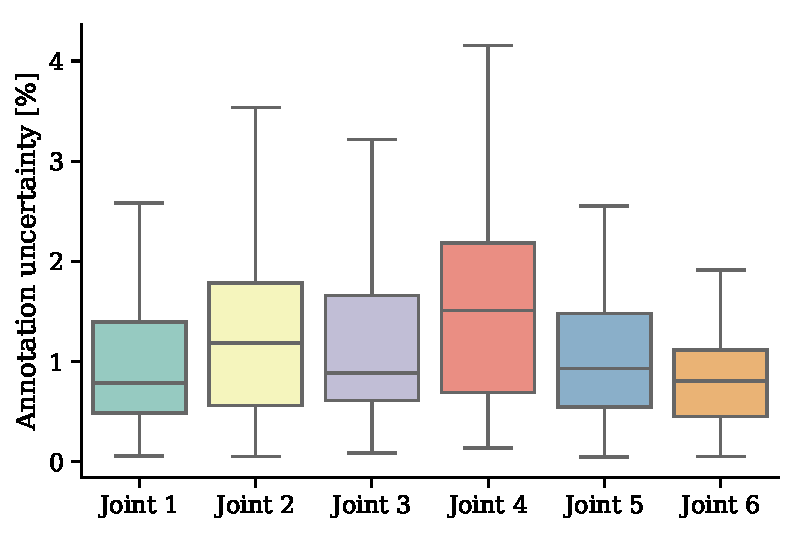
\includegraphics[width=\columnwidth]{figures/results/human_uncertainty/human_uncertainty.pdf}
            \caption {
                \label{fig:humanuncertainty} 
                Human uncertainty estimates in pose annotation. Results are in percent of image diagonal.
            }
        \end{subfigure}
        \begin{subfigure}[t]{0.49\columnwidth}
            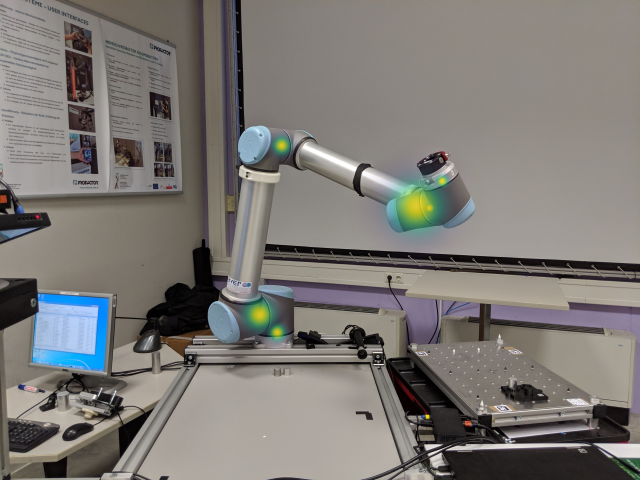
\includegraphics[width=\columnwidth]{figures/results/human_uncertainty/human_uncertainty_belief.png}
            \caption {
                \label{fig:humanuncertainty_belief} 
                Uncertainty estimates superimposed as Gaussian kernels on one of the images to be annotated.
            }
        \end{subfigure}
        \caption {
            \label{fig:uncertainty} 
            Uncertainty estimates from human annotation.
        }
    \end{figure}

    \subsection{Runtime Analysis}

\begin{table}[htbp]
\caption{Performance evaluation}
\begin{center}
\begin{tabular}{|c|c|}
\hline
\textbf{Blender instance} & \textbf{Runtime ms/batch} \\
\hline
1 & 103 ms ± 5.17 ms \\
\hline
2 & 43.7 ms ± 10.3 ms \\
\hline
\end{tabular}
\label{tab1}
\end{center}
\end{table}

\section*{Acknowledgment}

Work presented in this paper has received funding from the European Union’s Horizon 2020 research and innovation programme under grant agreement No 721362 (project “ZAero”).

\small
\bibliographystyle{ieeetr}
\bibliography{biblio}



%%%\begin{thebibliography}{00}
%%%\bibitem{b1} G. Eason, B. Noble, and I. N. Sneddon, ``On certain integrals of Lipschitz-Hankel type involving products of Bessel functions,'' Phil. Trans. Roy. Soc. London, vol. A247, pp. 529--551, April 1955.
%%%\bibitem{b2} J. Clerk Maxwell, A Treatise on Electricity and Magnetism, 3rd ed., vol. 2. Oxford: Clarendon, 1892, pp.68--73.
%%%\bibitem{b3} I. S. Jacobs and C. P. Bean, ``Fine particles, thin films and exchange anisotropy,'' in Magnetism, vol. III, G. T. Rado and H. Suhl, Eds. New York: Academic, 1963, pp. 271--350.
%%%\bibitem{b4} K. Elissa, ``Title of paper if known,'' unpublished.
%%%\bibitem{b5} R. Nicole, ``Title of paper with only first word capitalized,'' J. Name Stand. Abbrev., in press.
%%%\bibitem{b6} Y. Yorozu, M. Hirano, K. Oka, and Y. Tagawa, ``Electron spectroscopy studies on magneto-optical media and plastic substrate interface,'' IEEE Transl. J. Magn. Japan, vol. 2, pp. 740--741, August 1987 [Digests 9th Annual Conf. Magnetics Japan, p. 301, 1982].
%%%\bibitem{b7} M. Young, The Technical Writer's Handbook. Mill Valley, CA: University Science, 1989.
%%%\end{thebibliography}
%%%\vspace{12pt}
%%%\color{red}
%%%IEEE conference templates contain guidance text for composing and formatting conference papers. Please ensure that all template text is removed from your conference paper prior to submission to the conference. Failure to remove the template text from your paper may result in your paper not being published.

\end{document}
